\section{$\Delta$Q implementation}

Originally, $\Delta$Q(x) denotes the probability that an outcome occurs in a time $t \le x$, defining then the "intangible mass" of such IRV as $1 - \lim_{x\to\infty} \Delta Q (x)$.
We then extend the original definition to fit real time constraints, needing to calculate $\Delta$Qs continuously.

For a given probe, $\Delta$Q($t_l$, $t_u$, $dMax$) is the probability that the time of series with samples between time $t_l < t_u$, an outcome or probe occurs in time t $\le$ dMax.

\subsection{Internal representation of a $\Delta$Q}
    We provide a $\Delta$Q class to calculate the $\Delta$Q of a probe between a lower time bound $t_l$ and an upper time bound $t_u$.
    
    The $\Delta$Q can be calculated in various ways: 
    
    \paragraph{Observed $\Delta$Q}
    
    The first way is by having $n$ collected outcome instances between $t_l$ and $t_u$, calculating its PDF and then calculating the \textit{empirical cumulative distribution function} (ECDF) based on its PDF. This is called the \textbf{Observed $\Delta$Q}.
    
    \paragraph{Calculated $\Delta$Q}
    
    A $\Delta$Q can also be calculated by performing operations which are the result of outcome expressions on two or more $\Delta$Qs, the notion of outcome instances is then lost between calculations, as the interest shifts towards calculating the resulting PDFs and ECDFs. This is called the \textbf{Calculated $\Delta$Q}.
    
    Below, is how both are calculated given $n$ samples.
    
    \subsubsection{PDF}
  We approximate the PDF of the observed random variable $\textbf{X}$ via a histogram. We partition the values into $N$ bins of equal width, this is required to ease future calculations.
        Given $\lbrack x_i, x_{i+1} \rbrack$ the interval of a bin $i$, where $x_i = i\Delta x$, and $\hat{p}(x_i)$ the value of the PDF at bin $i$, for $n$ bins:
        \begin{equation}
            \begin{cases}
                \hat{p}(i) = \dfrac{n_i}{n}, \text{if } i \le n \\
                \hat{p}(i) = \hat{p}(n), \text{if } i > n \\
            \end{cases}
            \label{eq:pdf}
        \end{equation}
   With $n_i$ the number of successful samples whose elapsed time is contained in the bin $i$, $n$ the total number of samples.
    \subsubsection{ECDF}
    The value $\hat{f}(x_i)$ of the ECDF at bin $i$ with $n$ bins can be calculated as:
    \begin{equation}
        \begin{cases}
            \hat{f}(i) = \sum_{j=1}^{i} \hat{p}(j), & \text{if } i \le n \\  
            \hat{f}(i) = \hat{f}(x_n), & \text{if } i > n 
        \end{cases}
        \label{eq:cdf}
    \end{equation}
    
    \subsection{dMax}
        The key concept of $\Delta$QSD is having a maximum delay after which we consider that the execution is failed, this is represented in an observable as $dMax$. The user defines, for each observable the maximum delay its execution can have.

Setting a maximum delay for an observable is not a job that can be done one-off and blindly, it is something that is done with an underlying knowledge of the system inner-workings and must be thoroughly fine tuned during the execution of the system by observing the resulting distributions of the obtained $\Delta$Qs. 

We define in our oscilloscope a formula to dynamically define a maximum delay:
\begin{equation}
    dMax = \Delta_{t base} * 2^n * N  
    \label{eq:dMax}
\end{equation}
Where:
\begin{itemize}
    \item $\Delta_{t base}$ represents the base width of a bin, equal to 1ms.
    \item $N$ the number of bins.
\end{itemize}

The user must choose:
\begin{itemize}
    \item $n$: We define a range $\lbrack -10, 10 \rbrack$ for $n$. This gives a good enough range to account for all possible delays an user wishes to have.
    \item $N$: We define a range $\lbrack 1, 1000 \rbrack$ for $N$. This is a good enough bound to allow for finer grained bins, or less precision if needed. 
\end{itemize}

Some tradeoffs must though be acknowledged when setting these parameters, a higher number of bins corresponds to a higher number of calculations and space complexity, a lower $dMax$ may correspond to more failures. These are all tradeoffs that must be considered by the system engineer and set accordingly.
    \begin{figure}[H]
        \begin{center}
            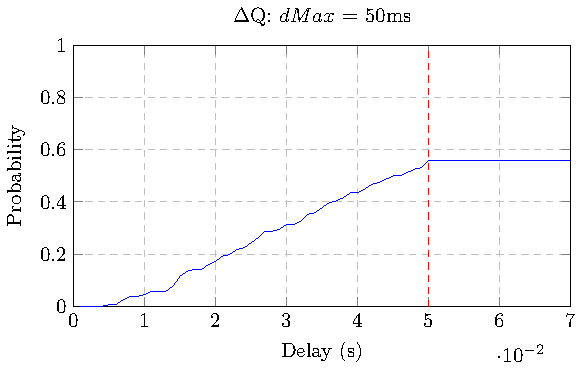
\includegraphics[scale = 1.2]{tikz/cdf_dmax.pdf}
        \end{center}
        \caption{$\Delta$Q: $dMax$ = 50ms, the CDF will stay constant when delay $> dMax$}
    \end{figure}

    \subsection{QTA}
        A simplified QTA is defined for probes. We define 4 points for the step function at 25, 50, 75 percentiles and the maximum amount of failures accepted for an observable. An observed $\Delta$Q will calculate that based on the samples collected. 

    \subsection{Operations}
    In a previous section we talked about the possible operations that can be performed on and between $\Delta$Qs, the time complexity of FTF, ATF and PC is trivially $\mathcal{O}(N)$ where N is the number of bins. As to convolution, the naïve way of calculating convolution has a time complexity of $\mathcal{O}(N^2)$, this quickly becomes a problem as soon as the user wants to have a more fine-grained understanding of a component. Below we present two ways to perform convolution.

        \subsubsection{Convolution}
        
        \paragraph{Naïve convolution}
        Given two $\Delta$Q binned PDFs $f$ and $g$, the result of the convolution $f \circledast g$ is given by 
        \begin{equation}
            (f \circledast g)\lbrack n \rbrack = \sum_{m = 0}^{N} = f\lbrack m \rbrack g \lbrack n - m \rbrack  
            \label{eq:discconv}
        \end{equation}
 
    \paragraph{Fast Fourier Transform Convolution}
        FFTW (Fastest Fourier Transform in the West) is a C subroutine library \cite{fftw3} for computing the discrete Fourier Transform in one or more dimensions, of arbitrary input size, and of both real and complex data. We use FFTW in our program to compute the convolution of $\Delta$Qs.
    
    Whilst the previous algorithm is far too slow to handle a high number of bins, convolution leveraging Fast Fourier Transform (FFT) allows us to reduce the amount of calculations to $\mathcal{O}(n \text{log} n)$. 
    
    FFT and naïve convolution produce the same results in our program barring $\varepsilon$ differences (around $10^{-18}$) in bins whose result should be 0.

    \subsubsection{Arithmetical operations}
        We can apply a set of arithmetical operations between $\Delta$Qs ECDFs, and on a $\Delta$Q.
    \paragraph{Scaling (multiplication)} A $\Delta$Q can be scaled w.r.t a constant $0 \le j \le 1$. It is equal to binwise multiplication on ECDF bins.
    \begin{equation}
        \hat{f_r}(i) = \hat{f}(i) \cdot j
        \label{eq:mul_ecdf}
    \end{equation}

    \paragraph{Operations between $\Delta$Qs} 
        Addition, subtraction and multiplication can be done between two $\Delta$Q of equal bin width (but not forcibly of equal length) by calculating the operation between the two ECDFs of the $\Delta$Qs:
        \begin{equation}
            \Delta \text{Q}_{AB}(i) = \hat{f_A}(i) [\cdot, +, -] \hat{f_B}(i)
            \label{eq:op_dq}
        \end{equation}
    \subsection{Confidence bounds}
    To observe the stationarity of a system we must observe a window of $\Delta$Qs of an observable and calculate confidence bounds over said windows. We present here the formulae required to give such bounds with 95\% confidence level. 
        For a bin $i$, its mean over a window is:
            \begin{equation}
                \mu_i = \dfrac{1}{n_i} \sum_{j=1}^{n_i} x_{ij}
                \label{eq:mean_ecdf}
            \end{equation}
        Where $x_{ij}$ is a bin's $i$ value for an ECDF $j$.
        Its variance:
            \begin{equation}
                \sigma^2_i = \dfrac{1}{n_i} \sum_{j=1}^{n_i} x^2_{ij} - \mu^2_i
                \label{eq:var_ecdf}
            \end{equation}
        The confidence intervals $CI_i$ for a bin $i$ can then be calculated as:
        \begin{equation}
            CI_i = \mu_i \pm z_{\alpha/2} \cdot \dfrac{\sigma_i}{\sqrt{n_i}}      
            \label{eq:ci_i}
        \end{equation}
    The bounds can be updated dynamically by inserting or removing a $\Delta$Q, this allows us to consider a small window of execution rather than observing the whole execution.
        \begin{figure}[H]
            \begin{center}
                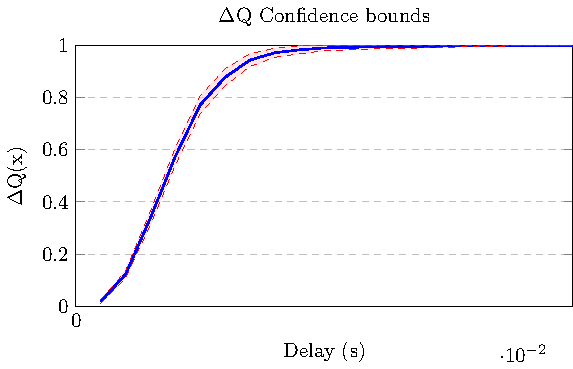
\includegraphics[scale=1.2]{tikz/ci.pdf} 
            \end{center}
            \caption{Upper and lower bounds of the mean of multiple $\Delta$Qs. In a system that behaves linearly, the bounds will be close to the mean, once the overload is approaching, or a system is showing behaviour that diverges from a linear one, the bounds will be larger.}
        \end{figure}
    \subsection{Rebinning}
        Rebinning refers to the aggregation of multiple bins of a bin width $i$ to another bin width $j$. 
        Operations between $\Delta$Qs can be done on $\Delta$Qs that have the same bin width, this is why it is fundamental that all observables have a common $\Delta_{tbase}$. This allows for fast rebinning to a common bin width. \\
        Given two $\Delta$Qs $\Delta$Q$_i$, $\Delta$Q$_j$:
        \begin{center}
            $\Delta_{Tij}$ = max \{$\Delta_{Ti}, \Delta_{Tj} \}$
        \end{center}
        and the PDF of the rebinned $\Delta$Q at bin $b$, from the original PDF of $n$ bins, where $k$ = $\frac{\Delta{_Ti}}{\Delta_{Tj}}$:
        \begin{equation}
            p'_b = \sum_{n=b \cdot k}^{b+ 1 \cdot k - 1} p_n, \quad b=0,1,\dots \lceil \frac{N}{k} \rceil  
        \end{equation}
        We perform rebinning to a higher bin width for a simple reason, while this leads to loss of information for the bin with the lowest bin width, rebinning to a lower bin width would imply inventing new values for the $\Delta$Q with the highest bin width.
       
        \begin{figure}[H]
            \begin{center}
                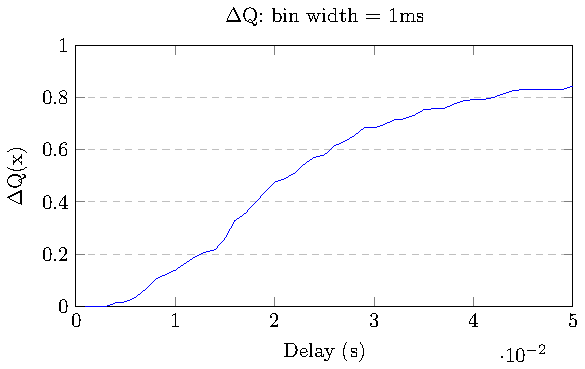
\includegraphics[scale=1.2]{tikz/cdf.pdf}
            \end{center}
            \caption{Sample $\Delta$Q with 1ms bins}
        \end{figure}%
 
        \begin{figure}[H]%
            \begin{center}
                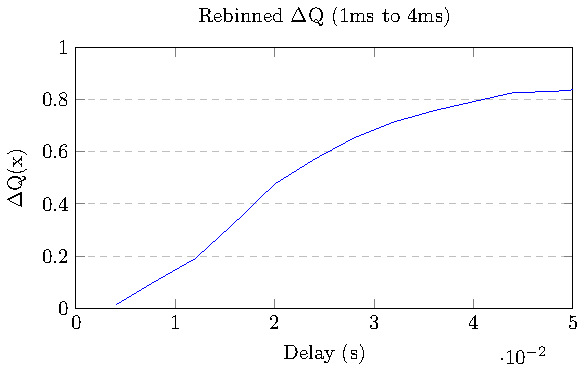
\includegraphics[scale=1.2]{tikz/rebinned_cdf.pdf}
            \end{center}
            \caption{Previous $\Delta$Q after rebinning to 4ms bins}
        \end{figure}%
